\begin{tikzpicture}[arj/.style={-latex}] 
\begin{scope}[start chain=R going right,
    pp/.style={on chain,join=by arj,label=below:{#1}}]
 \path node[pp=424 x 424 x 3]{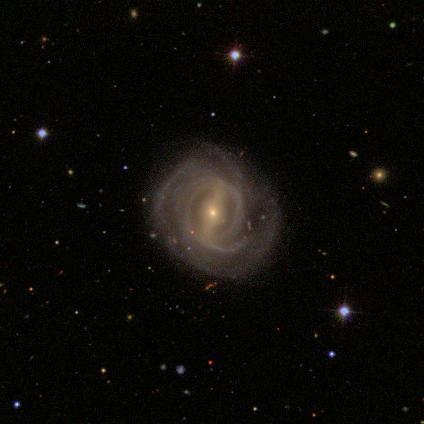
\includegraphics[width=2.7cm]{images/Data_Augmentation/405615.jpg}}
  node[pp=\small256 x 256 x 3]{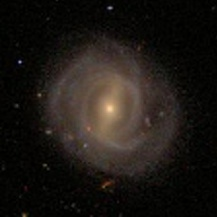
\includegraphics[width=2.4cm]{images/Data_Augmentation/centre_crop.jpg}}
  [arj/.append style={opacity=0}]
  node[pp,minimum width=2cm]{}
  node[pp,minimum width=2cm]{}  
  [arj/.append style={opacity=1}]
  node[pp=Flipping,opacity=1]{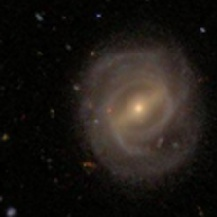
\includegraphics[width=2cm]{images/Data_Augmentation/flipping.jpg}}
  node[pp=Brightness,opacity=1]{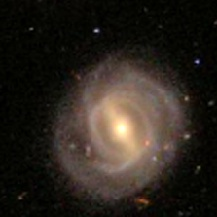
\includegraphics[width=2cm]{images/Data_Augmentation/brightness.jpg}}
  ;
\end{scope} 
\pgfmathtruncatemacro{\matindexA}{3}
\pgfmathtruncatemacro{\matindexB}{4}
\path (R-\matindexA) node[matrix,label=below:Random Rotation] {
    \node(R-\matindexA-1){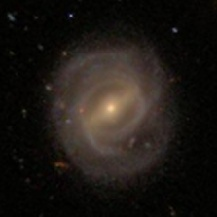
\includegraphics[width=2cm]{images/Data_Augmentation/rotate_1.jpg}};\\
    \node(R-\matindexA-2){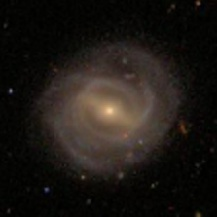
\includegraphics[width=2cm]{images/Data_Augmentation/rotate_2.jpg}};\\
   \node(R-\matindexA-3){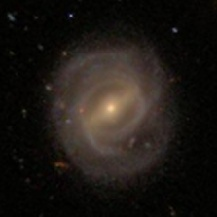
\includegraphics[width=2cm]{images/Data_Augmentation/rotate_3.jpg}};\\
\node(R-\matindexA-4){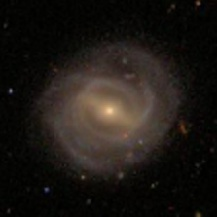
\includegraphics[width=2cm]{images/Data_Augmentation/rotate_4.jpg}};\\}
   (R-\matindexB) node[matrix,label=below:Height and width shift] {\node[xscale=-1](R-\matindexB-1){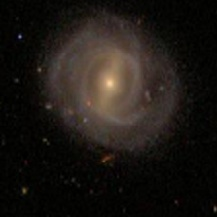
\includegraphics[width=2cm]{images/Data_Augmentation/height_shift.jpg}};\\
   \node[yscale=-1](R-\matindexB-2){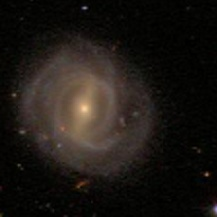
\includegraphics[width=2cm]{images/Data_Augmentation/width_shift.jpg}};\\};
\path[arj] (R-\the\numexpr\matindexA-1\relax.east) foreach \X in {1,...,4} { edge (R-\matindexA-\X.west)}   
 (R-\matindexA.east) foreach \X in {1,2} { edge (R-\matindexB-\X)};   
\end{tikzpicture}